\documentclass[dvipdfmx]{jsarticle}

\usepackage[utf8]{inputenc}
\usepackage{graphicx}
\usepackage{float}
\usepackage{amsmath}
\begin{document}
\title{人工知能 課題番号09  \\Wuの定理の実装}
\author{電気電子工学科 03-180500\\ 平井雄太}
\date{2018年11月5日}
\maketitle

\section{プログラムの使い方}
本課題では、Wuの定理に基づく幾何の自動定理証明システムを実装した。プログラムの簡単な使い方と注意すべき点を以下に記す。

\subsection{必要な実行環境}
python3

sympy(python用のライブラリ)

以上がインストールされている必要がある。

\subsection{基本的な使い方}
本プログラムは以下のように使用する。まず、単にプログラムを実行したいだけであれば、
\begin{quote}
\$python3 Wu.py 
\end{quote}
と入力する。すると仮定と結論を入力するように促されるので、それらを入力し、最後に空行を入力するWuの手続きを実行する。この時、数式の入力はpythonの入力形式に則るものとする。例えば,$x^2$は$x**2$と入力する。ここで、\underline{変数はアルファベット大文字小文字の1文字のみが許される。}また、変数を使用する際には、\underline{アルファベットの小さい順から使用しなくてはならない}ので注意が必要である。例えば、変数に"x1"などは使えないし、変数として(a, b, d)などを用いてはならない。
\subsection{従属変数の選定}
デフォルトでは、従属変数はアルファベット順に小さい方から仮定の数の分だけ選んだものが使用される。例えば仮定の数が全部で7個であれば,従属変数として
\begin{quote}
(a, b, c, d, e, f, g)
\end{quote}
が従属変数として使用される。個別に従属変数を設定するには以下のようにする。例えば
\begin{quote}
(b, c, f, g, j, i, h)
\end{quote}
を従属変数として用いるには
\begin{quote}
\$python3 Wu.py --vars b,c,f,g,j,i,h
\end{quote}
とすればいい。ただし\underline{変数間に空白を含めてはいけない}。また、\underline{変数の数は仮定の数と同じにする必要があり}、\underline{同じ変数を重複させて含めてはいけない}。

\subsection{外部ファイルからの読み取り}
外部ファイルから仮定と結論を読み取ることが可能である。最初に仮定を、最後の1行に結論を記入しておく。例えば, Pythagollas.txtに
\begin{quote}
a*c+b*d

a**2+b**2+c**2+d**2-(a-c)**2-(b-d)**2
\end{quote}
という式が格納されていたとする。この時、プログラムは
\begin{quote}
\$python3 Wu.py --file Pythagollas.txt 
\end{quote}
と入力することにより実行される。

\subsection{その他}
\begin{quote}

\$python3 Wu.py --latex
\end{quote}
とすることで,数式を{\LaTeX}形式で出力することが可能である。
また、
\begin{quote}
\$python3 Wu.py --help
\end{quote}
と入力することで簡単な説明を見ることができる。
\clearpage
\section{本プログラムを用いたいくつかの定理の証明}
本プログラムを用いていくつかの定理の自動証明を行なった。なお、これらの定理の仮定と結論の式は全てテキストファイルとして添付してある。
    \subsection{ピタゴラスの定理}
        \begin{figure}[H]
            \centering
            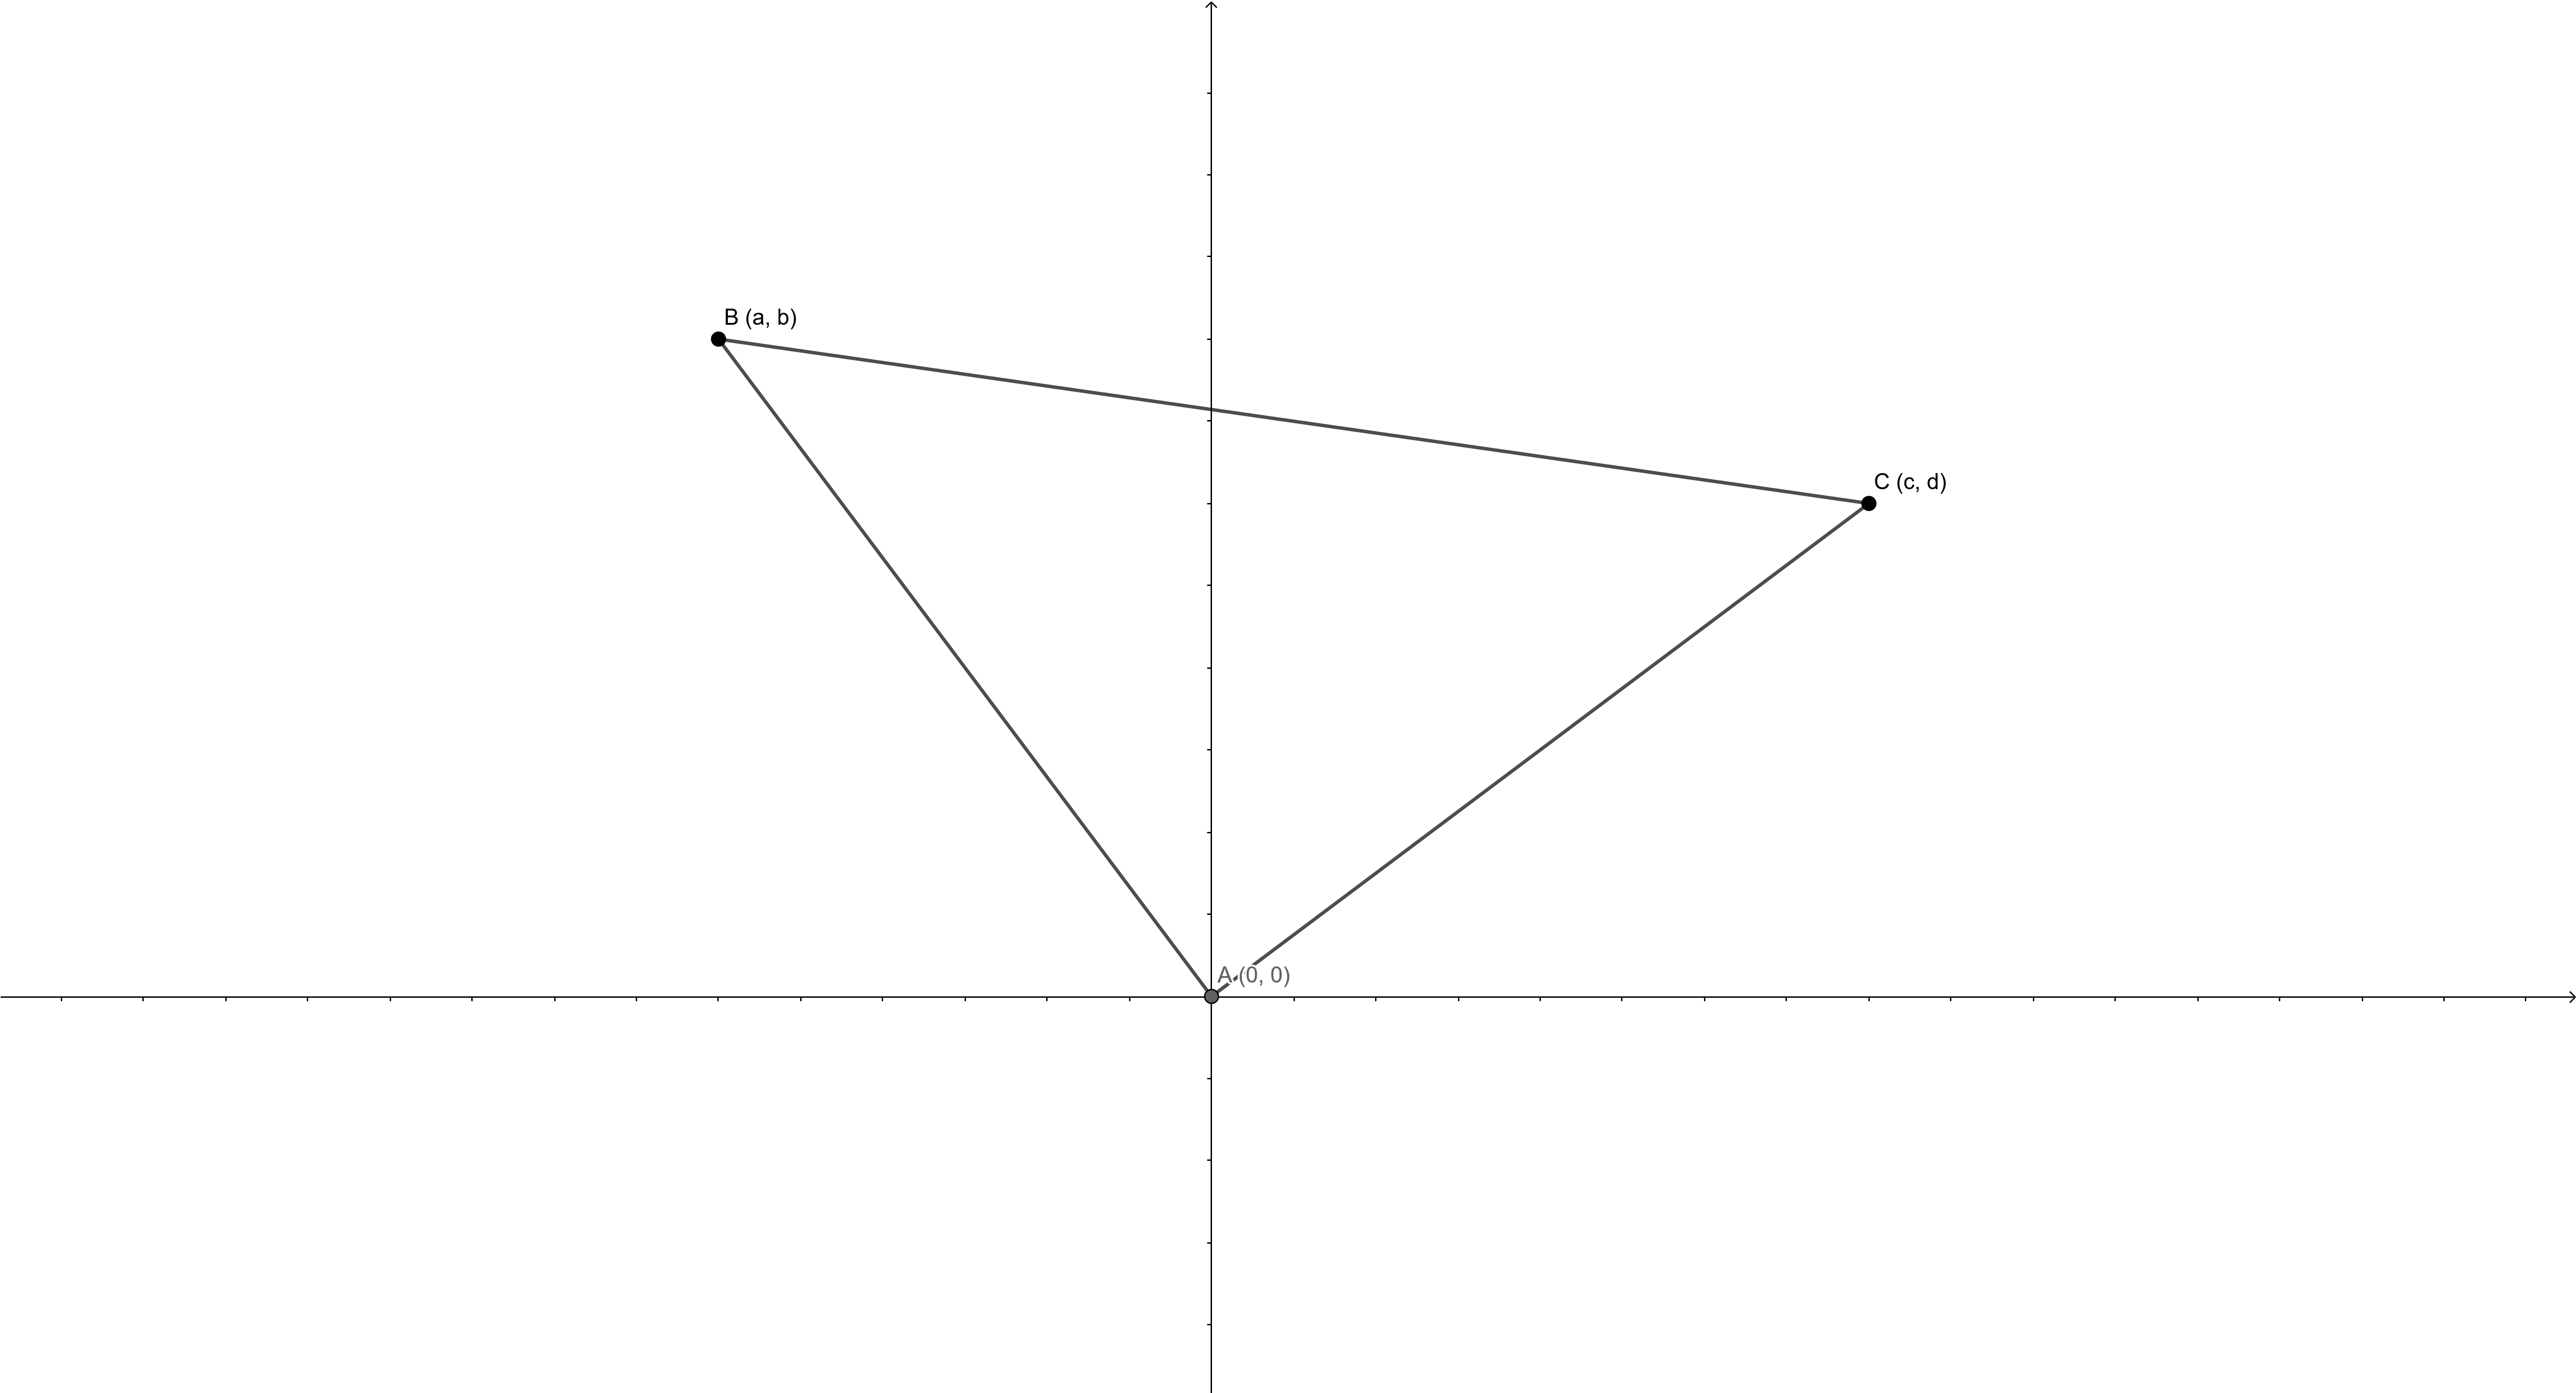
\includegraphics[width=10cm]{Pythagoras.png}
            \caption{ピタゴラスの定理}
            \label{fig:Pythagoras}      
        \end{figure}

        
        \begin{table}[H]
            \label{table:PythagorasAssumption}
            \centering
            \caption{ピタゴラスの定理の仮定と結論の式}
            \begin{tabular}{cc}
                仮定 & 結論 \\
                \hline \hline
                $Hyp_{1} = a c + b d$ & ABとACは垂直\\
                $Conc =a^{2} + b^{2} + c^{2} + d^{2} - \left(a - c\right)^{2} - \left(b - d\right)^{2}$ & $BC^2=AB^2+AC^2$ \\
            \end{tabular}
        \end{table}

        \begin{figure}[H]
            \centering
            \label{fig:PythagorasTri}
            \fbox{$
                \begin{aligned}
                    Tri_{1}(a) = a c + b d
                \end{aligned}
            $}
            \caption{ピタゴラスの定理の三角形式}
        \end{figure}

        \begin{figure}[H]
            \centering
            \label{fig:PythagorasWu}
            \fbox{$
                \begin{aligned}
                    Rem_{0} &= a^{2} + b^{2} + c^{2} + d^{2} - \left(a - c\right)^{2} - \left(b - d\right)^{2}\\
                    Rem_{1} &= 0\\
                    Subsidaries &= c
                \end{aligned}$}
            \caption{ピタゴラスの定理のWuの手続きの実行過程}            
        \end{figure}

    \subsection{角の二等分線の定理}
\end{document}

























